% Maria -- moved for better placement
\begin{figure*}[ht]
  \centering
  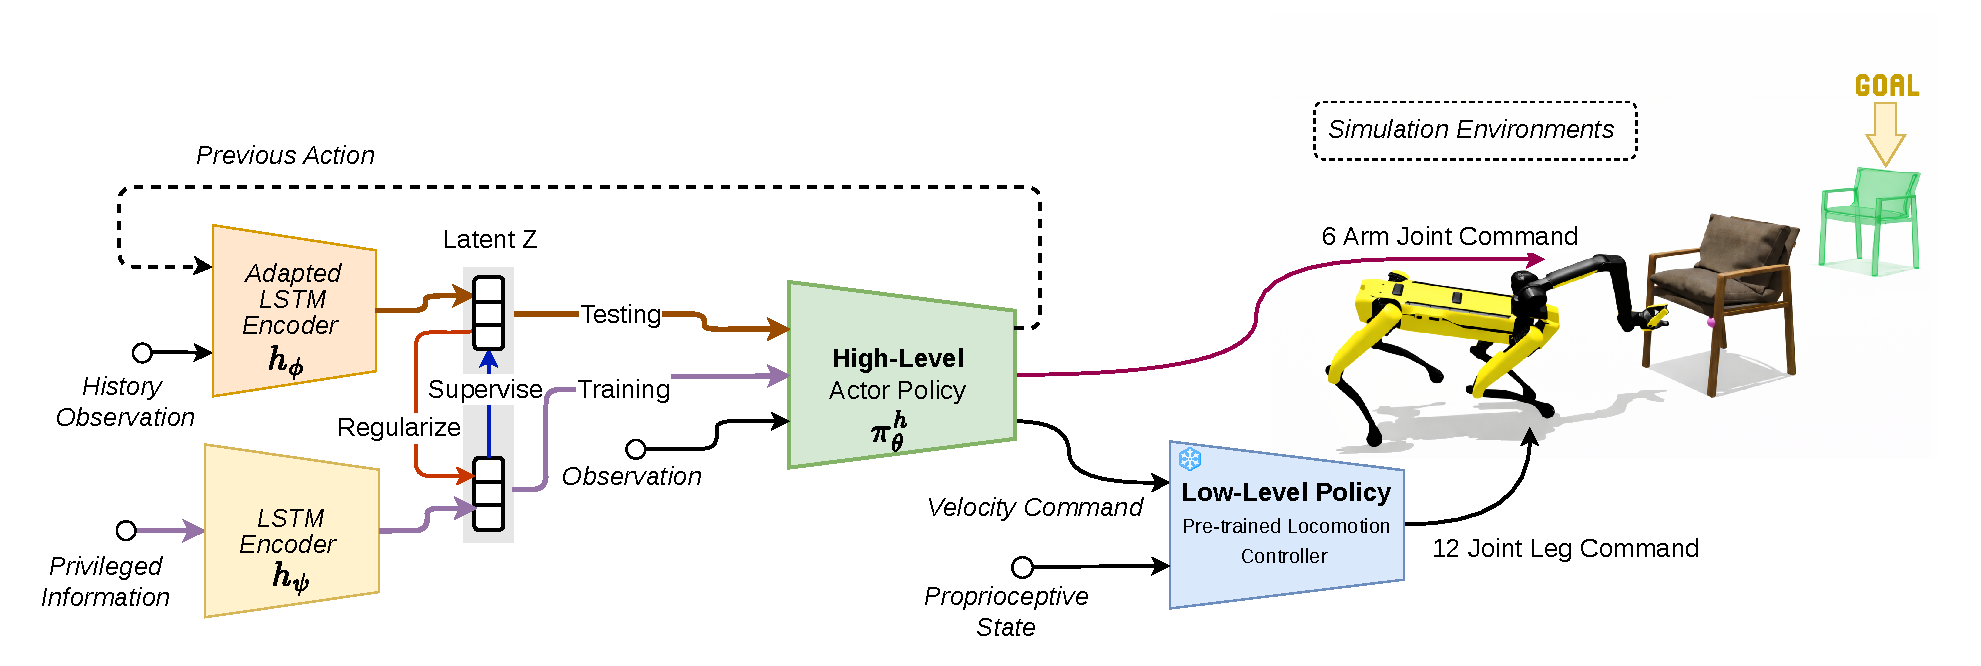
\includegraphics[width=0.9\textwidth]{Images/systemdiagram-Page-4.drawio (1).pdf}
  \caption{\textbf{Hierarchical pushing pipeline.} A high-level policy outputs %task 
  actions for the base and arm. During training, a privileged encoder produces a latent embedding \(z\) that regularizes and supervises a history-based encoder used at test time. The high-level policy generates base velocity commands and arm joint targets; base commands are executed through a pretrained low-level locomotion controller (conditioned on proprioception), while arm commands are applied directly. Both whole-body and arm-mediated pushing are trained/evaluated in the same %simulation 
  environments with identical goals and object sampling.}
  \label{fig:system}
\end{figure*}

%--------------------------------------------------
\section{Methods}
\label{sec:methods}

The task in this work is goal-directed non-prehensile pushing with a quadrupedal mobile manipulator, where the objective is to move an object to a desired SE(2) pose by manipulating it in SE(3) space. We study two contact modalities: \textit{whole-body pushing (WB)}, which uses base/torso contacts, and \textit{arm-mediated pushing (AM)}, which uses end-effector/arm contacts while coordinating locomotion.



Motivated by hierarchical control and adaptation frameworks \cite{Kumar2021RMA,2025relic}, we propose a two-level architecture for non-prehensile locomotion–manipulation pushing that integrates goal-conditioned object motion with contact acquisition and regulation (Fig.~\ref{fig:system}). The overall control process has two levels. A high-level controller generates task-specific commands, while a pretrained low-level controller tracks these commands via joint-level actuation. Depending on the different contact modalities, the motion commands fed to the low-level controller %to track 
also differ: 
\begin{itemize}[leftmargin=*]
    \item \textbf{Whole-Body pushing}: the high-level policy outputs a SE(2) base velocity command expressed in the robot body frame. 
\begin{equation}
a_t^{\text{WB}} = [v_x,\ v_y,\ \omega_z] \label{eq:wb-command}
\end{equation}
where $v_x, v_y$ are linear velocities and $\omega_z$ angular velocity. 
\item \textbf{Arm-Mediated Pushing}: The policy produces a compact whole-body command that integrates base motion, body regulation, and arm control,
\begin{equation}
a_t^{\text{AM}} = \left[
v_x,\ v_y,\ \omega_z,\ q^{\text{arm}}_{1:6}
\right] \label{eq:am-command}
\end{equation}
where the first three are velocity terms and $q_{1:6}^{arm}$ denotes the target joint positions for the six arm joints. In our experiments, the gripper configuration is fixed.
\end{itemize} 

% =========================
% Low-level controller
% =========================

\subsection{Low-level Locomotion Controller}
The low-level locomotion controller receives task-specific commands from the high-level controller and predicts joint-position targets $q_t\in \mathbb{R}^{12}$ for the quadruped legs. They are converted into torque commands 
$\tau$ via a leg impedance controller for the robot to execute. The low-level controller is pretrained and then frozen during training of the high-level controller for the target non-prehensile pushing task, thereby decoupling gait stabilization from task-level exploration and improving training stability.

\noindent \textbf{Whole-body pushing (WB)}: For WB, the frozen low-level locomotion policy receives the base velocity commands predicted by the high-level controller and produces joint-position targets at the low-level control rate for the robot to reach. We use a pretrained quadruped locomotion policy that tracks commanded planar base velocities, as in prior work \cite{Rudin2021WalkMinutes}. This policy is \emph{frozen} after pretraining and serves as the low-level stabilizer for all WB experiments.

\begin{figure}[t]
    \centering
    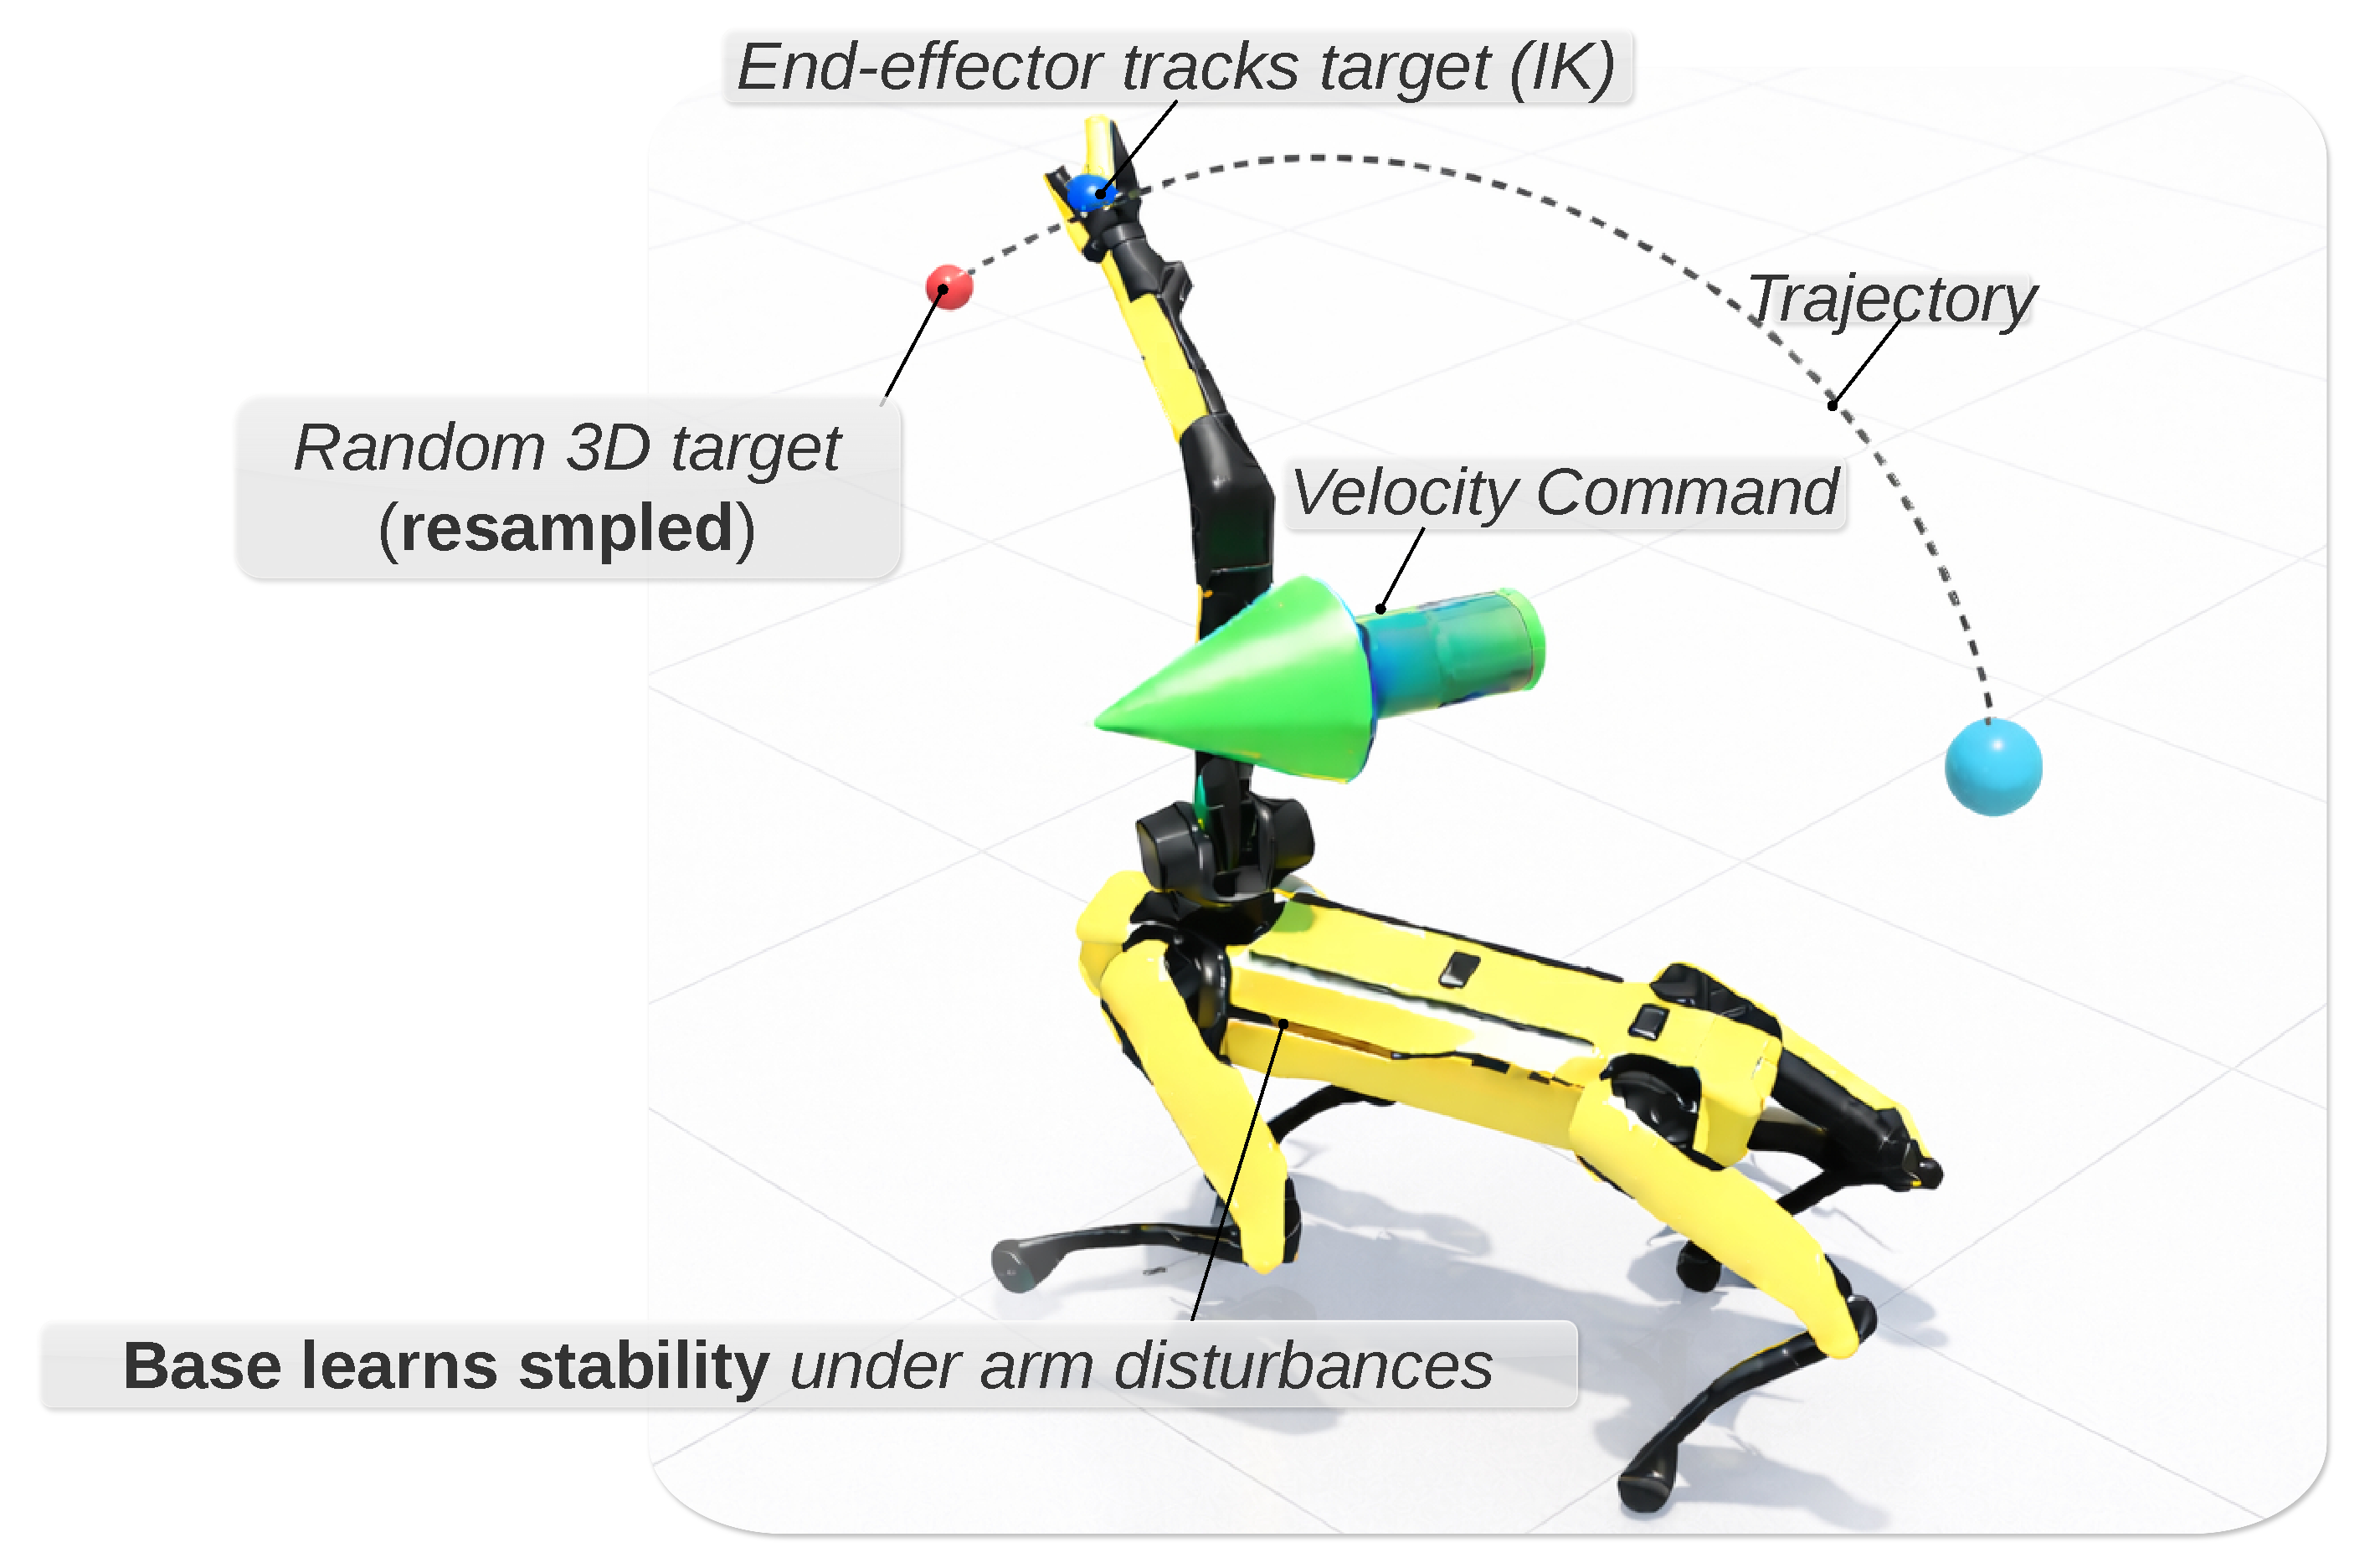
\includegraphics[width=0.67\linewidth]{Images/systemdiagram-Page-5.drawio-4.pdf}
    \caption{\textbf{Low-level locomotion prior pretraining.}
    Spot is trained to locomote while the arm tracks randomly resampled 3D end-effector targets (red), producing diverse arm motions and disturbances; the resulting locomotion policy is then frozen and used as a stabilizing prior for pushing.}
    \label{fig:lowlevel_relic_training}
    \vspace{-0.6em}
\end{figure}



\noindent \textbf{Arm-mediated pushing (AM)}: For AM, the frozen low-level locomotion policy receives the compact control commands mentioned in Equation (\ref{eq:am-command}) and predicts joint-level targets that maintain both base stability and collision-free arm configurations. Inspired by \cite{2025relic}, we pretrain our own custom locomotion policy in simulation. At training time, 3D target poses for the robot's end-effector are sampled randomly within the observation space using inverse kinematics (IK). We then train a locomotion policy using PPO \cite{schulman2017proximalpolicyoptimizationalgorithms} to command the robot to move its end-effector to track those sampled poses (Fig.~\ref{fig:lowlevel_relic_training}). This sampling process yields a wide distribution of arm configurations to train the prior locomotion policy and improve the robustness of our pretrained policy to variations in upper-body configurations. After pretraining, the resulting locomotion policy is \emph{frozen} and used as the stabilizing layer in all AM pushing experiments.





% =========================
% High-level Policy
% =========================
\subsection{High-level Controller}
\label{subsec:high-level-control}
The high-level controller generates task-level commands that enable the robot to achieve the goal-directed pushing objective. It comprises two components. First, to capture both temporal dependencies and environmental variations, we adopt an encoder module $h_{\psi}$ \cite{fu2022deepwholebodycontrollearning} to encode available information into a structured latent representation. The resulting latent representations are fused and provided to the high-level policy actor $\pi^h_{\theta}$, which predicts task-appropriate actions conditioned on the latent features and the current observation. 

\subsubsection{Encoder Module}
Inspired by Regularized Online Adaptation (ROA) \cite{fu2022deepwholebodycontrollearning}, the encoder module consists of a teacher encoder and a student encoder in the simulation environment. They are both implemented as Long Short-Term Memory (LSTM) networks \cite{hochreiter1997long}. During training, the teacher encoder $h_\psi$ takes the privileged information history $\{\xi_t^1, \dots, \xi_t^{N-1}, \xi_t^N\}$ as input and predicts a latent vector $z_\psi \in \mathbb{R}^{16}$. Here, $N=24$ denotes the horizon size, and the privileged information vector $p_t^i$ encodes all environmental settings, including the object mass, the static friction coefficient on the ground, etc (see Table~\ref{tab:domain_rand}). The student encoder $h_\phi$ is trained to estimate the latent vector $z_\phi$ conditioned solely on the history of observations and actions, without any access to the privileged information. The teacher $h_\psi$ and the student $h_\phi$ are trained simultaneously, with the adaptation loss:
\begin{equation}
\label{eq:adapt}
L_{adapt}=  \lambda \| z_\phi - \text{sg}[z_\psi] \|^2 + \| \text{sg}[z_\phi] - z_\psi \|^2
\end{equation}
where $\text{sg}[\cdot]$ denotes the stop-gradient operator, and $\lambda$ is the Lagrangian multiplier for regularization.
\subsubsection{High-level Actor Policy}
Conditioned on the latent vector $z_\psi\in \mathbb{R}^{16}$ and the current observation, the high-level actor policy $\pi_{\theta}^h$ is to predict high-level task-specific motion commands described in Equation (\ref{eq:wb-command}) and (\ref{eq:am-command}) for the pretrained low-level controllers to execute. We adopt an end-to-end model-free reinforcement learning hierarchy to train the actor policy, i.e. update the model parameters to maximize the desired reward:
\begin{equation}
    J(\pi_\theta^h, \pi^l, h_\psi) = \mathbb{E}_{r \sim p(r \mid \pi^h_\theta, \pi^l, h_\psi)}\left[ \sum_{t=0}^{T-1}\gamma^t r_t \right] \label{eq:ppo}
\end{equation}
where $\gamma$ is the discounting factor and $r_t$ refers to the reward terms discussed in \ref{sec:reward}. We optimize it with PPO \cite{schulman2017proximalpolicyoptimizationalgorithms} using the default hyperparameter settings provided by the RSL-RL library \cite{schwarke2025rsl}.

% =========================
% Observations
% =========================

\subsection{High-level Controller Observations}
\label{sec:obs}
Observations to the high-level controller include robot proprioception and task state. The exact observation set depends on the contact modality (WB vs.\ AM) and is summarized in Table~\ref{tab:obs_combined}.

% =========================================
% Combined observation table (WB vs AM)
% =========================================
\begin{table}[ht]
\centering
\caption{\textbf{High-level policy observations.} Dimensions for whole-body (WB) and arm-mediated (AM) modalities.}
\label{tab:obs_combined}
\scriptsize
\setlength{\tabcolsep}{4pt}
\renewcommand{\arraystretch}{1.08}
\begin{tabular}{lcc}
\toprule
\textbf{Observation term} & \textbf{WB dim.} & \textbf{AM dim.} \\
\midrule
Base linear velocity ($v_{\text{base}}$) & 3 & 3 \\
Base angular velocity ($\omega_{\text{base}}$) & 1 & 3 \\
Projected gravity ($g_{\text{base}}$) & 3 & 3 \\
Previous action ($a_{t-1}$) & 3 & 9 \\
\addlinespace[0.25em]\hline\addlinespace[0.15em]
Robot--object relative vector & 2 (xy) & -- \\
Object--goal relative vector & 2 (xy) & 3 \\
Object--goal distance ($d_{bg}$) & 1 & -- \\
Pushable heading in base frame & 2 & -- \\
Goal heading in base frame & 2 & -- \\
End-effector to object vector & -- & 3 \\
Object rotation in base frame & -- & 9 ($R_{bo}$) \\
Goal rotation in object frame & -- & 9 ($R_{og}$) \\
\addlinespace[0.25em]\hline\addlinespace[0.15em]
Object planar velocity in base frame & 2 (xy) & -- \\
Speed toward goal ($v_{\parallel g}$) & 1 & -- \\
Tangential speed ($v_{\perp g}$) & 1 & -- \\
Arm joint positions (relative) & -- & 6 \\
Arm joint velocities & -- & 6 \\
\addlinespace[0.25em]\hline\addlinespace[0.15em]
Low-level prior obs (frozen) & 48 & 84 \\
Privileged encoder & 16 & 16 \\
\bottomrule
\end{tabular}
\vspace{-0.6em}
\end{table}




% =========================
% Our key novelty: interaction intent sampling + curriculum
% =========================
\subsection{Contact-Point Sampling Strategy in AM}
\label{sec:sampling}

Training the high-level controller for the arm-mediated pushing (AM) task requires the policy to learn both \emph{where} and \emph{how} to establish contact across diverse object geometries. The approach in \cite{dadiotis2025dynamic} samples candidate points from a single planar surface, which is effective for objects with large flat regions but does not generalize to geometrically complex objects, such as chairs, carts, and tables (see Figure~\ref{fig:unseen_object_set}) considered in our pipeline. To address this limitation, we propose a contact-point sampling strategy that generates a valid surface contact point for each training episode. This strategy promotes a consistent object approach and interaction without relying on hand-crafted features or object-specific heuristics. The strategy consists of four steps: 
% =========================
% Fig: cached point-cloud target pipeline (one-column)
% =========================
\begin{figure}[ht]
  \centering
  \includegraphics[width=0.75\columnwidth]{Images/mesh_point_clould.pdf}
  \caption{\textbf{Contact-point sampling strategy in training AM task} For each object, we cache a dense surface point cloud offline.
  At the start of the training episode, we filter the cloud to a reachable, interaction-rich subset. We sample a single target point $p_{\text{tgt}}$, which
  is transformed to the world frame and used as a reach/contact intent for AM.}
  \label{fig:chair_target_sampling_pipeline}
\end{figure}
\begin{enumerate}
    \item \textit{Point candidate sampling on the object surface}: For each object mesh (USD asset in IsaacLab \cite{Baginski2025IsaacLab}), we generate a dense set of surface samples and treat them as contact-point candidates. We then uniformly sample a subset $\mathcal{S}$ from these surface points prior to training.
    \item \textit{Point Candidate Filtering}: At the beginning of each training episode for AM, we refine the candidate point set $\mathcal{S}$ to obtain a subset $\mathcal{S}_{\text{int}}$ through a filtering process based on three criteria. Specifically, we enforce: (i) \textbf{reachability}, by excluding points located within the interior of the object surface; (ii) \textbf{collision-avoidance}, by removing points positioned too close to the ground that could result in unintended collisions; and (iii) \textbf{smoothness}, by favoring points situated on relatively large, planar, and easily accessible surface regions. 
    % This filtering procedure ensures that the selected contact points are physically feasible, safe for interaction, and conducive to stable pushing behavior.
    \item \textit{Contact Point Guidance}: During the training of the arm-mediated pushing (AM) policy, we randomly sample a point $p_{contact}$ from the filtered set $\mathcal{S}_{\text{int}}$ to serve as the designated contact location on the object surface. This point specifies the position at which the robot is expected to position its end-effector to initiate the pushing task. To promote accurate and consistent reaching behavior for the end-effector, we introduce a \emph{reach reward} $r_{reach}$ (see Table~\ref{tab:am_reward_terms}). This reward term encourages the policy to minimize the reaching error and facilitates stable contact establishment prior to pushing.
    \item \textit{Adaptive Weight Finetuning for Reach Reward}: As training progresses and the end-effector consistently approaches the selected contact point $p_{contact}$, it becomes desirable for the policy to shift its focus from precisely reaching $p_{contact}$ to the primary pushing objective. Continuing to focus on optimizing $r_{reach}$ at this stage may hinder the optimization of the robot's behavior to push the object. To address this issue, we adopt an adaptive weighting scheme that reduces the weight of $r_{reach}$ once the end-effector is sufficiently close to $p_{contact}$ after 2000 training iterations. 
    % This mechanism enables a smooth transition from contact acquisition to effective object manipulation.
\end{enumerate}




% =========================
% Rewards + safety constraints
% =========================
\subsection{Task-specific Reward Design}
\label{sec:reward}
The reward terms designed to train the high-level actor policy generally reflect three goals: (i) task completion (to push the object to the target pose),
(ii) stability (to encourage smooth robotic motions), and (iii) safety (to avoid collisions or object toppling).


\paragraph{WB reward}
We adopt the reward formulation proposed in \cite{Jeon2023WholeBodyQuadruped}. In general, this design promotes successful task completion by penalizing the distance between the object and the designated goal, while simultaneously discouraging unstable behaviors through regularization of action velocities. Such a structure balances task performance with motion stability, leading to smoother manipulation behaviors.
% Concretely, we use a shaped WB reward written as a weighted metric vector:
% \begin{equation}
% \footnotesize
% \label{eq:wb_reward_condensed}
% r_t^{\mathrm{WB}}=
% \Big\langle
% w^{\mathrm{WB}},
% \begin{bmatrix}
% \clip\!\big(d_{bg}(t\!-\!1)-d_{bg}(t),-\delta,\delta\big)\\[0.1em]
% \big(\max(0,-\hat u_{rb}(t)^{\!\top}\hat u_{bg}(t))\big)^2\\[0.1em]
% \exp\!\big(-d_{bg}(t)^2/\sigma_{xy}^2\big)\ +\ \mathbf{1}\!\Big[\sum_{i=t-K+1}^{t}\mathbf{1}_{\text{succ}}(i)=K\Big]\\[0.1em]
% \clip\!\big(\cos\theta(t),0,1\big)\ -\ \mathbf{1}\!\big[\cos\theta(t)<\cos\theta_{\min}\big]\\[0.1em]
% -\|a_t-a_{t-1}\|_2^2
% \end{bmatrix}
% \Big\rangle ,
% \end{equation}
% \noindent where $w^{\mathrm{WB}}$ is a fixed weight vector that balances progress, approach geometry, precision, %/settling, 
% stability, and smoothness.


\paragraph{AM reward}
AM uses a pose-matching objective (we use a keypoint-based pose error \cite{Jeon2023WholeBodyQuadruped} for robustness to different object shapes), plus a reach reward that encourages the end-effector toward the sampled intent $p_{contact}$ from \ref{sec:sampling}. We also penalize undesirable contacts between the robot body (other than the arm) and the objects, and regularize action rates to promote smooth, safe behaviors. More details can be found in Table~\ref{tab:am_reward_terms}. We utilize a curriculum learning strategy, downscaling the reaching reward weight to 0.63 after 2000 iterations and upscaling the sparse completion reward weight to 4.0 after 4000 iterations. To formalize our task, let $\mathbf{K}_{\text{object}}$ and $\mathbf{K}_{\text{goal}}$ denote the Cartesian coordinates of the object and goal keypoints, respectively. We define $p_{ee}$ as the position of the end-effector and target region, $\theta_{tilt}$ as the object's inclination angle, and $F_b$ as the magnitude of the contact force applied to robot body $b$. The orientation error between the current object state and the goal state is denoted by $\Delta\theta$. Furthermore, we establish tolerance thresholds of $d_{tol} =$ 5 cm and $\theta_{tol} =$ 5°. Finally, $\mathbf{1}(\cdot)$ represents a standard indicator function that evaluates to 1 if the specified condition is met, and 0 otherwise.

% We use a curriculum design. The weight of reaching reward is downscaled to 0.63 after 2000 iterations. The weight of sparse completion reward is upscaled to 4.0 after 4000 iterations. We denote the cartesian coordinates if the keypoints corresponding to the object and its goal as $\mathbf{K}_{\text{object}}$ $\mathbf{K}_\text{{goal}}$, respectively. We define $p_{ee}$ as the position for the end-effector and target region. We define $\theta_{tilt}$ as the object's inclination angle. We define $F_b$ as the magnitude of the contact force applied to a specific robot body $b$. We define $\Delta\theta$ as the difference in orientation between the current object state and the goal state. We define $d_{tol}$ to be 5cm, $\theta_{tol}$ to be $5^\circ$. The $\mathbf{1}(\cdot)$ represent an indicator function that evaluates to 1 if the condition inside is true, and 0 otherwise.

% ---------------- AM reward terms (style-matched) ----------------
% \subsubsection{Arm-mediated pushing reward structure.}
% \begin{table}[ht]
% \centering
% \caption{\textbf{Arm-mediated pushing (AM): reward terms.}}
% \label{tab:am_reward_terms}
% \scriptsize
% \setlength{\tabcolsep}{3pt}
% \renewcommand{\arraystretch}{1.10}
% \begin{tabular}{@{}p{2.0cm}p{\dimexpr\columnwidth-2.0cm-0.55cm-4\tabcolsep\relax}p{0.55cm}@{}}
% \toprule
% \textbf{Term} & \textbf{Definition} & \textbf{$w$}\\
% \midrule
% \multicolumn{3}{@{}l}{\textit{Goal pose + progress}}\\
% Pose match &
% $r_{\text{pose}}=\exp\!\big(-e_{\text{kp}}^{2}/\sigma_3^{2}\big)$
% & 3.0\\
% Reach shaping &
% $r_{\text{reach}}=\exp\!\big(-\|p_{ee}-p_{\text{tgt}}\|^{2}/\sigma_1^{2}\big)$
% & 2.5\\
% Velocity to goal &
% $r_{\text{vel}}=\exp\!\big(-(1-\alpha)^{2}/\sigma_2^{2}\big)$
% & 0.156\\
% \addlinespace[0.20em]\midrule\addlinespace[0.10em]
% \multicolumn{3}{@{}l}{\textit{Stability + safety}}\\
% Object stability &
% $r_{\text{stab}}=\sigmoid\!\big(s(\cos\theta-\cos\theta_{\lim})\big)$
% & 0.4\\
% Undesired contacts &
% $r_{\text{col}}=-\sum_{b\in\mathcal{B}_{\neg ee}}\mathbf{1}\!\left[\|F_b\|>\tau\right]$
% & -0.05\\
% \bottomrule
% \end{tabular}
% \end{table}
% \begin{table}[ht]
% \centering
% \caption{\textbf{Arm-mediated pushing (AM): reward terms.}}
% \label{tab:am_reward_terms}
% \resizebox{\columnwidth}{!}{%
% \renewcommand{\arraystretch}{1.2}
% \begin{tabular}{@{}llcccc@{}}
% \toprule
% \textbf{Term} & \textbf{Definition} & \textbf{$w$} & \textbf{$\sigma$} & \textbf{Curriculum} & \textbf{Iterations} \\
% \midrule
% Keypoints alignment & $R_{pose} = \exp\left(-\frac{\| \mathbf{K}_{goal} - \mathbf{K}_{obj} \|_2}{\sigma^2}\right)$ & 4.0 & 0.78 & -- & -- \\
% Reach & $r_{\text{reach}}=\exp\left(-\|p_{ee}-p_{\text{target}}\|^{2}/\sigma^{2}\right)$ & 2.5 & 0.60 & 2.50 $\to$ 0.63 & 1500 \\
% Velocity to goal & $r_{\text{vel}}=\exp\left(\frac{\hat{\mathbf{v}}_{object} \cdot \hat{\mathbf{d}}_{goal}}{\sigma^2} - 1\right)$ & 0.16 & 0.71 & -- & -- \\
% Object stability & $r_{\text{stab}}=\frac{1}{1 + \exp\left(500 \cdot (\theta_{\text{tilt}} - 20^\circ)\right)}$ & 0.40 & -- & -- & -- \\
% Undesired contacts & $r_{\text{col}}=-\sum_{b\in\mathcal{B}_{\neg ee}}\mathbf{1}\!\left[\|F_b\|>0.2\right]$ & 0.05 & -- & -- & -- \\
% Sparse completion & $\mathbf{1} \left( \| \mathbf{p}_{\text{goal, xy}} - \mathbf{p}_{\text{push, xy}} \|_2 \le d_{\text{tol}} \land \Delta\theta \le \theta_{\text{tol}} \right)$ & 0.00 & -- & 0.00 $\to$ 4.00 & 4000 \\
% Action rate & $R_{rate\_exp} = \exp\left( -\frac{\| \mathbf{a}_t - \mathbf{a}_{t-1} \|_2^2}{\sigma^2} \right)$ & 0.3 & 0.35 & -- & -- \\
% Action Regularization & $R_{accel} = \exp\left( -\frac{\| \mathbf{a}_t - 2\mathbf{a}_{t-1} + \mathbf{a}_{t-2} \|_2^2}{\sigma^2} \right)$ & 0.3 & 0.38 & - & - \\
% \bottomrule
% \end{tabular}%
% }
% \end{table}

\begin{table}[ht]
\centering
\caption{\textbf{Arm-mediated pushing (AM): reward terms.}}
\label{tab:am_reward_terms}
\resizebox{\columnwidth}{!}{%
\renewcommand{\arraystretch}{1.2}
\begin{tabular}{@{}llcc@{}}
\toprule
\textbf{Term} & \textbf{Definition} & \textbf{$w$} & \textbf{$\sigma$} \\
\midrule
Keypoints alignment & $R_{pose} = \exp\left(-\frac{\| \mathbf{K}_{goal} - \mathbf{K}_{obj} \|_2}{\sigma^2}\right)$ & 4.0 & 0.78 \\
Reaching & $r_{\text{reach}}=\exp\left(-\|p_{ee}-p_{\text{target}}\|^{2}/\sigma^{2}\right)$ & 2.5 & 0.60 \\
Velocity to goal & $r_{\text{vel}}=\exp\left(\frac{\hat{\mathbf{v}}_{object} \cdot \hat{\mathbf{d}}_{goal}}{\sigma^2} - 1\right)$ & 0.16 & 0.71 \\
Object stability & $r_{\text{stab}}=\frac{1}{1 + \exp\left(500 \cdot (\theta_{\text{tilt}} - 20^\circ)\right)}$ & 0.40 & -- \\
Undesired contacts & $r_{\text{col}}=-\sum_{b\in\mathcal{B}_{\neg ee}}\mathbf{1}\!\left[\|F_b\|>0.2\right]$ & 0.05 & -- \\
Sparse completion & $\mathbf{1} \left( \| p_{o} - p_g \|_2 \le d_{\text{tol}} \land \Delta\theta \le \theta_{\text{tol}} \right)$ & 0.10 & -- \\
Action rate & $R_{rate\_exp} = \exp\left( -\frac{\| \mathbf{a}_t - \mathbf{a}_{t-1} \|_2^2}{\sigma^2} \right)$ & 0.3 & 0.35 \\
Action regularization & $R_{accel} = \exp\left( -\frac{\| \mathbf{a}_t - 2\mathbf{a}_{t-1} + \mathbf{a}_{t-2} \|_2^2}{\sigma^2} \right)$ & 0.3 & 0.38 \\
\bottomrule
\end{tabular}%
}
\end{table}


% Xun we need to remove this section entirely. Its uncessary... We are already talking about it in the expremeint section.. 
% For me, it's better to place it here. Anyway, I will not try to change it. 


% % =========================
% % Training + Randomization (brief; full specs in Experiments)
% % =========================
% \subsection{Random Initialization \& Training}
% \label{sec:training_summary}

% The training environment is implemented in IsaacLab~\cite{Baginski2025IsaacLab}. At the beginning of each episode, the robot, the manipulated object, and the goal pose are randomly initialized within an $8\mathrm{m} \times 8\mathrm{m}$ planar arena. To enhance policy robustness and generalization, we further apply domain randomization to object dynamics and initial conditions, including parameters such as mass and friction coefficients.
% Our training objective is to optimize Equation (\ref{eq:adapt}) and (\ref{eq:ppo}). All remaining numerical settings for the experimental protocol (e.g., $N_{\text{env}}$, episode horizon, control rates, and randomization ranges)
% are reported Tables~\ref{tab:setup_summary}--\ref{tab:domain_rand}. The set of object categories evaluated in our experiments is summarized in Table~\ref{tab:object_sets}. 